\cotefile{64}
\scanpage{2}
I \hfill Fourbis combinatoires

\margin{(40)}(ens. à 4 éléments, carrés, octaèdres, modules libres de rang $2$ sur $\mathbb{Z}/4\mathbb{Z}$).
% archive sheet number: 1
\scanpage{3}\mspage{\unsure{1}}
1. Ens. à quatre éléments.

Un ens. à quatre éléments $I$ est muni canoniquement d'une structure \deleted{\unsure{de torseur sous un}} \inserted{d'espace affine de} dim $2$ sur $\mathbb{F}_2$, i.e. d'un sous-groupe $V\subset\unsure{\mathfrak{S}|G}_I$, isomorphe (non can!) à $\mathbb{F}_2^2$, tel que l'action de $V$ sur \deleted{$\unsure{\mathbb{F}_2}$} $I$ en fasse un torseur. Le sous-groupe $V\subset\mathfrak{S}_I$ est le seul sous-groupe distingué abélien $\ne\{0\}$, \deleted{\unsure{c'est aussi}} il est son propre \deleted{normalisateur} \inserted{centralisateur} i.e. $\mathfrak{S}_I/V$ opère fidèlement sur $V$, en fait on a
\[
\mathfrak{S}_I/V\xrightarrow{\sim}\mathrm{Aut}_{\mathrm{gr}}(V)=\mathrm{Aut}_{\mathbb{F}_2\text{-vect}}(V)\xrightarrow{\sim}\deleted{\mathrm{Aut}}\mathfrak{S}_J
\]
où $J=V^{\unsure{\times|*}}$, la suite exacte
\[
1\longrightarrow V\longrightarrow\mathfrak{S}_I\longrightarrow\mathfrak{S}_J\longrightarrow1
\]
étant \deleted{\unsure{isomorphe|identique}} \inserted{identique} à la suite
\[
1\unsure{\text{---}|\longrightarrow}\underset{\text{translations}}{V}\longrightarrow\mathrm{Aut}_{\mathrm{aff}}(I)\longrightarrow\mathrm{Aut}_{\mathbb{F}_2}(V)\longrightarrow1.
\]

Les \inserted{trois} éléments de $J=V^{\times}$ correspondent aux trois partitions de type $(2.2)$ de $I$
% slanted
\margin{ou aux trois involutions \unsure{sur|en} $I$ sans pt fixe}
(on peut l'interpréter \inserted{ainsi,} que les éléments de $J$ correspondent aux \uline{droites} \inserted{vectorielles} de $V^{*}$, qui définissent \deleted{\unsure{des|les}} donc des \deleted{\illegible{1}} relations d'équivalence de $I$, vers les espaces affines quotients de dim $1$) -- les classes \unsure{intervenant|inversement} dans l'ensemble de ces \inserted{3} relations d'équivalence correspondent aux $6$ \deleted{\unsure{applications|paires}} \inserted{parties} à deux éléments de $I$) ou aussi \deleted{\unsure{aux}} $6$ droites affines de l'espace affine $I$, l'application
\[
\begin{aligned}
\mathcal{P}_2(I)&\longrightarrow\mathcal{P}_{\unsure{2,2|1,1}}(\unsure{I|J})\\
A&\longmapsto\{A,I\setminus A\}
\end{aligned}\tag*{1}
\]
% archive sheet number: 2
\scanpage{4}
s'identifiant à l'application qui associe à tte droite affine de $I$ sa \uline{direction}, qui est une droite de l'espace des translations $V$. La fibre d'un $\unsure{j|J|i}\in\mathcal{P}_{2,2}(I)$, i.e. \unsure{l'ens|l'un} des \deleted{\illegible{1}} deux classes \inserted{de cette partition}, est donc l'espace quotient $I/(D_{\unsure{j|i}}=\{0,\unsure{j|J}\})$

Le foncteur ``oubli de la structure'' qui va de la \deleted{\unsure{une}} catégorie des espaces affines de dim $2$ sur $\mathbb{F}_2$, vers la cat. des ensembles à quatre éléments
% slanted
\margin{on prend comme flèches les flèches \uline{inversibles}}
\[
\mathrm{Aff}_2(\mathbb{F}_2)\xrightarrow{\approx}(\mathrm{Ens}_4)
\]
est une équivalence de catégories -- et \inserted{$=$ un iso, si on définit la notion d'espace affine sur $\mathbb{F}_2$ par la donnée d'une structure sur \deleted{\unsure{$I$}} \inserted{(donnée d'un sous-groupe de $\unsure{\mathfrak{S}|G}_I$ peut être)} sur un $I$ \deleted{tout} seul}

Je dis que le foncteur
\margin{\unsure{id}}
\[
\begin{aligned}
(\mathrm{Ens}_4)&\longrightarrow(\mathrm{Gr})\\
I&\longmapsto\mathfrak{S}_I
\end{aligned}
\]
est pleinement fidèle, ou encore que pour tt $I$, $\mathfrak{S}_I$ a \deleted{\unsure{le}} un centre trivial et tout automorphisme de $\mathfrak{S}_I$ est intérieur. \deleted{\unsure{Pour|Pourrais}} \inserted{\unsure{(Il}} suffirait bien sûr de l'énoncer pour $\mathfrak{S}_4$ ?).

On va définir pour ceci un foncteur quasi-inverse
\[
\deleted{(\mathrm{Ens}}(\mathrm{Gr})'\longrightarrow(\mathrm{Ens}_4)
\]
sur l'image essentielle $(\mathrm{Gr})'$ des groupes isomorphes à $\mathfrak{S}_4$. Si on a un tel groupe $G$, on considère l'ens \deleted{\unsure{de ses}} \inserted{des} \deleted{\unsure{groupes conjugués}} \inserted{3-sous-\unsure{gr. maximaux|groupes} de} Sylow, il y en a exactement quatre ! Pour préciser ce point et \unsure{récupérer|réexprimer|récapituler}
% archive sheet number: 3
\scanpage{5}\mspage{2}
la structure de torseur sur cet ens, on considère le sous-groupe abélien distingué \deleted{\unsure{et}} non nul $V$ de $G$, de sorte que $V$ \deleted{\unsure{soit}} est un vectoriel de rang $2$ sur $\mathbb{F}_2$, et $G/V\xrightarrow{\sim}\mathrm{Aut}_{\mathbb{F}_2}(V)$, et on note que les \inserted{3-}sous-groupes de Sylow de $G$ correspondent aux ``relèvements'' de l'unique 3-sous-groupe de Sylow de $G/V\simeq\unsure{\mathfrak{S}|G}_J$. ($J=V^\times$), savoir $\mathfrak{S}_J^+=[\mathfrak{S}_J,\mathfrak{S}_J]$, d'indice $2$ dans $\mathfrak{S}_J$. \deleted{\unsure{Comme}} L'ens. $I_G$ des 3-sous-groupes de Sylow de $G$ s'identifie donc à l'ens des scindages de l'extension
\[
\cdot\quad\unsure{1\text{---}|\vdash|1\longrightarrow} V\unsure{\text{---}|\longrightarrow} G^+\longrightarrow\mathfrak{S}_J^+\unsure{\text{---}|\longrightarrow}1
\]
du 3-groupe $\mathfrak{S}_J^+$ par le 2-groupe $V$. Sur l'ens de ses scindages, $V$ opère donc transitivement par autom. intérieurs, d'ailleurs $V^{\mathfrak{S}_J^+}=\{0\}$ ($\mathfrak{S}_J^+$ est le groupe des permutations circulaires sur $V^\times=J$), donc $I_G$ est bien un torseur sous $V$.

Quand on part de $\unsure{J|I}$ et \deleted{$\unsure{\mathfrak{S}}$} $G=\mathfrak{S}_I$, on trouve une bijection
\[
\begin{aligned}
I&\unsure{\text{---}|\longrightarrow} I_G\\
i&\longmapsto\mathfrak{S}_{I\setminus\{i\}}^+=\text{l'unique 3-ss-gr. de Sylow}\\
&\hspace{8em}\text{de }\mathfrak{S}_I\text{ qui fixe }i
\end{aligned}
\]
Ainsi \deleted{\unsure{les deux foncteurs}} \inserted{les} foncteurs $I\unsure{\text{---}|\longrightarrow|\longmapsto}\mathfrak{S}_I$, $G\unsure{\text{---}|\longrightarrow|\longmapsto} I_G$, et la comparaison $I\longrightarrow I(\mathfrak{S}_I)$, on a un iso avec le \deleted{l'identité} foncteur identique,
% archive sheet number: 4
\scanpage{6}
Pour le \unsure{composé|compos.} dans l'autre sens, on trouve que $G$ opère sur l'ens $I_G$ de ses trois ss-groupe de Sylow par autom. intérieurs, d'où
\[
G\xrightarrow{\sim}\unsure{\mathfrak{S}|G}_{I_G}
\]
qui est un iso.

Éléments de $\mathfrak{S}_I$.

a) $1$

b) Les \inserted{trois} éléments \deleted{non nuls de} \inserted{de} $V^{*}$, qui forment une orbite $J$ sous $\mathfrak{S}_I$, et correspondent aux élém. de $\mathcal{P}_{22}(I)$
% slanted
\margin{``translations'' (non nulles) [sym. p.r. aux trois axes du cube]}

c) Les \deleted{\unsure{deux}} $8$ éléments d'ordre $3$, se répartissent en \deleted{quatre} \inserted{deux} \deleted{torseurs} paquets de $4$ qui sont des torseurs (à gauche ou à droite, au choix) sous $V$, suivant les deux éléments $\ne1$ de $\mathfrak{S}_J^+$, L'ens de ces éléments s'identifie aussi à $I\times\underline{\omega}$, où $\underline{\omega}=\omega(\unsure{J|I})\bigl(\simeq\omega(I)\bigr)$, par l'application qui associe à tout $\unsure{\rho|p}\in\mathfrak{S}_I$ d'ordre $3$ son unique pt fixe dans $I$ (ou encore, le sous-groupe de Sylow qu'il engendre), \uline{et} l'orientation qu'il détermine \deleted{\unsure{via son}} ou encore son image dans $\mathfrak{S}_J^+$.
% slanted
\margin{``rotations'' (ayant un pt fixe et un seul, lequel transforme $I$ en vectoriel \unsure{isom.} à $V$) [``rotations-sommets'' du cube]}

d) Les \deleted{\unsure{12}} \inserted{$6$} éléments \deleted{\unsure{non}} \inserted{d'ordre 2} de $\mathfrak{S}_I$ qui s'envoient dans $\mathfrak{S}_J^-$, en correspondance 1-1 avec l'ens $\mathcal{P}_2(I)$ -- ce sont les \uline{transpositions} dans $I$ qui se groupent \deleted{par} \inserted{en 3} \deleted{\unsure{gr}} paires, pour tte transposition $\tau_A$, $\tau_{A'}$ \deleted{$\unsure{\tau}$} $(A'=I\setminus A)$ est l'unique \inserted{autre} élément d'ordre $2$ tel que $\tau_A\tau_{A'}\in V^*$.
% slanted
\margin{``réflexions'' (ayant chacune une \deleted{\unsure{hyperplan}} droite de pts fixes) [``rotations-arêtes'' du cube]}

e) Les $6$ éléments d'ordre $4$ de $\mathfrak{S}_I$, correspondent aux $6$ ordres circulaires sur $I$. Pour
% slanted
\margin{[``rotations-faces'' du cube]}
% archive sheet number: 5
\scanpage{7}\mspage{3}
\deleted{\unsure{On}} on a $u^2\in V^*$, donc on a une application
\[
\mathrm{Circ}(I)\longrightarrow V^*
\]
de degré $2$. (qui définit donc une structure de \uline{cube}, ayant $V^\times$ comme ens des directions de faces, $\mathrm{Circ}(I)$ comme l'ens des six faces -- en fait ce cube est canoniquement orienté, cf plus bas.
% slanted
\margin{$\circledast$ On peut dire aussi que les six éléments d'ordre $4$ se répartissent par paires $\{\unsure{u},u^{-1}\}$ suivant les trois sous-groupes cycliques d'ordre $4$ \deleted{\unsure{de}} $G=\unsure{\mathfrak{S}|G}_I$, en corr. biunivoque (\unsure{via leurs élts d'ordre 2}) avec \deleted{\unsure{les}} les élts de $V^*$.}
% slanted
\margin{$I$ est l'ens des quatre diagonales du cube,}

L'isom canonique
\[
\underline{\omega}(I)\simeq\underline{\omega}(J)\tag*{$(\unsure{\omega|\alpha|*|**})$}
\]
On a
\[
\mathfrak{S}_{I\,\mathrm{ab}}\xrightarrow{\sim}\mathfrak{S}_{J\,\mathrm{ab}}\simeq\{\pm1\}
\]
les isom. étant donnés par la signature, d'où la possibilité de définir un iso. \deleted{\unsure{can}} \inserted{fonctoriel} $(\omega)$, dont le choix reste soumis cependant à convention (deux choix possibles). Quand on fixe un élément $i\in I$, alors on a
\[
\underline{\omega}_{\unsure{1|i}}(I)\xrightarrow{\sim}\underline{\omega}(\underbrace{I\setminus\{i\}}_{\simeq J})\deleted{\unsure{\times\{i,I\setminus\{i\}\}}}
\]
en associant à tt ordre \inserted{total} de \deleted{$\unsure{J}$} l'ordre \deleted{\unsure{induit}} \inserted{total} de $I$ qui sur $J$ est l'ordre donné, et qui admet $i$ comme \uline{premier} élément (la convention opposée aurait été de prendre $i$ comme \uline{dernier} élément).

\diagram{\begin{tikzcd}[ampersand replacement=\&,row sep=7pt,column sep=5pt,cells={nodes={font=\scriptsize}},execute at end picture={
\draw ([xshift=-2pt,yshift=7pt]opening.north west) .. controls ([yshift=13pt]source.north) and ([yshift=12pt]star.north) .. ([yshift=9pt]cyclic.north east);
\draw ([xshift=-3pt,yshift=5pt]mark.north west)--([xshift=-2pt,yshift=-2pt]norm.south west);
\draw[line width=.8pt] ([xshift=-6pt,yshift=-1pt]mark.north west)--([xshift=-8pt,yshift=-3pt]mark.north west)--([xshift=-7pt,yshift=-4pt]mark.north west);
}]
|[alias=opening]|\ast \&
|[alias=source]|V^*\arrow[r,shift left=2pt,"{x\mapsto\mathrm{Cent}_G(x)}","{\sim}" description] \&
\substack{\text{Sous-groupes}\\\text{cycliques}\\\text{d'ordre }4\\\text{de }G=\mathfrak{S}_I}\arrow[l,shift left=2pt,"{\sim}"'] \&
|[alias=mark,xshift=-1pt,yshift=-8pt]|\unsure{x|\ast}\arrow[d,start anchor=south east,end anchor=north west] \&
|[alias=star]|\substack{V^*\\\deleted{\illegible{1}}}\arrow[rr,leftrightarrow]\arrow[dr,start anchor=south east,end anchor=north west] \& {} \&
|[alias=cyclic]|\substack{\text{Ss-groupes cycliques}\\\text{d'ordre }4\text{ de }G=\mathfrak{S}_I}\arrow[dl,leftrightarrow]\\
\&\substack{\text{l'unique}\\\text{élément }\unsure{\ne|\#}1\\\text{de }\Gamma\cap V}
\& \Gamma\arrow[l,maps to]
\& |[alias=norm,xshift=4pt]|\mathrm{Norm}
\& D\mapsto\substack{\deleted{\unsure{\mathrm{Cent}(D)}}\\\text{élément}\\\text{non nul}\\\text{du centre}\\\text{de }D}\arrow[u,start anchor=north east,end anchor=south west]
\& \substack{\text{Ss-groupes de}\\\text{Sylow }\deleted{\unsure{2}}\text{ de }G=\mathfrak{S}_I\\D)} \&
\end{tikzcd}}
% archive sheet number: 6
\scanpage{8}
2. Structure\deleted{\unsure{s}} de carré combinatoire.

Le carré peut se définir, soit (dans le contexte des polygônes généraux) par un système
\[
(\underset{\text{sommets}}{S},\ \underset{\text{arêtes}}{A},\ \underset{\text{incidence}}{R})\tag*{(1)}
\]
satisfaisant les axiomes connus, soit (en utilisant l'\unsure{autom|autre} ``antipodisme'' $\underline{a}$ de $Q$) en termes de
\diagram{\begin{tikzcd}[ampersand replacement=\&,column sep=small,row sep=small]
\& S\arrow[d,"{\text{degré }2}"]\&\\
\text{(2)}\&\underset{(\simeq S/\underline a)}{D}\&\substack{\text{ens des diagonales}\\\text{(de card. 2)}},
\end{tikzcd}}
% slanted
\margin{Ou encore comme un ens. $S$ de cardinal $4$, avec une involution donnée sans pt fixe i.e. une \unsure{partition} de type $2,2$}
\deleted{\unsure{déf}} comme une famille de deux ensembles (les diagonales) de cardinal $2$ \deleted{\unsure{s}}, soit dualement \deleted{\unsure{pour|par}} en termes de
\diagram{\begin{tikzcd}[ampersand replacement=\&,column sep=small,row sep=small]
\& A\arrow[d,"{\text{degré }2}"]\&\\
\text{(3)}\&\underset{(\simeq A/\underline a)}{C}\&\substack{\text{ens des}\\\text{codiagonales}}
\end{tikzcd}}
% slanted
\margin{\unsure{id|ou ?}}
comme une \uline{autre} famille de deux ens. (les codiagonales \inserted{ou paires de \deleted{\unsure{côtés}} \unsure{côtés} opposés}) de cardinal $2$ \deleted{\unsure{s}}. Chacune des descriptions (1) (2) (3) est valable pour décrire le carré -- la première est \deleted{symétrique} \inserted{autoduale}, les \deleted{\unsure{deuxième|dernières|dimensions}} \inserted{deux autres} ne le sont pas, l'une privilégiant le point de vue ``sommets'', l'autre le point de vue ``arêtes'', comme ens de base (aussi dans l'un et l'autre cas c'est un ens. à quatre éléments avec involution ss \unsure{points|pts}
% archive sheet number: 7
\scanpage{9}\mspage{4}
fixes qui porte la structure\ldots). On peut aussi décrire ces structures en termes de $S$ ou de $A$ par la donnée d'un groupe $R$ (``forme'' de $\mathbb{Z}/4\mathbb{Z}$) opérant sur $S$ resp. sur $A$, qui devient un torseur sous $\Gamma$
\[
 S\text{ torseur sous }\Gamma\tag*{(2 bis)}
\]
\[
 A\text{ torseur sous }\Gamma\tag*{(3 bis)}
\]
ce qui fait finalement \deleted{quatre} \inserted{cinq} descriptions de \deleted{\unsure{la}} $=$ structure de ``carré''. Je veux expliciter les passages de l'une de ces descriptions à l'autre.

$\left.\begin{aligned}2\text{ bis})&\longmapsto2)\\3\text{ bis})&\longmapsto3)\end{aligned}\right\}$
en prenant l'unique élément $\underline a$ d'ordre $2$ de $\Gamma$, qui est une \unsure{d'involution|d'une involution|involution} ss pts fixes de $S$ (resp $A$), et on pose
\[
D=S/\underline a,\quad\text{resp. }C=A/\underline a
\]

$2)$\deleted{bis}$\implies1)$ \quad Soit $A\subset\mathcal{P}_2(S)\inserted{\subset\mathcal{P}(S)}$ défini par $A=\mathcal{P}_2(S)\setminus\mathrm{Im}\,D$, c'est un ens. à $4$ éléments, \deleted{qui} et on a une relation tautologique $R\subset S\times A$

$3)\implies1)$ \quad Soit $S\subset\mathcal{P}_2(A)$ défini par $S=\mathcal{P}_{\unsure{2}}(A)\setminus\mathrm{Im}\,C$, ens à $4$ éléments et on a relation tautologique $R'\subset A\times S$ d'où $ {}^{s}R'\stackrel{\mathrm{déf}}{=}R\subset S\times A$

$\left.\begin{aligned}1&\implies2\text{ bis}\\1&\implies3\text{ bis}\end{aligned}\right)$
On considère $\unsure{\mathfrak{D}|\mathscr{D}}=\mathrm{Aut}\underbrace{Q}_{Q=\{S,A,R\}}$
\diagram{\begin{tikzcd}[ampersand replacement=\&,row sep=small]
\&\unsure{\mathfrak{S}|G}_S\\
\deleted{\unsure{\mathfrak{D}_Q|\mathfrak{S}_Q|\mathfrak{D}}}\arrow[ur,hook]\arrow[dr,hook]\&\\
\&\mathfrak{S}_A
\end{tikzcd}}
\deleted{\unsure{on a|ou}} \deleted{\unsure{de} $\mathfrak{D}\unsure{\cap|{}_{A},} V_Q$} \inserted{ordre $8$} \inserted{2-sous-gr. de Sylow de $\mathfrak{S}_S$ ou $\mathfrak{S}_A$}
L'image inverse de $V_S\subset\mathfrak{S}_S$ et celle de $V_A\subset\mathfrak{S}_A$ \deleted{\unsure{sont}} deux $=$ sous-groupes d'ordre $4$ \deleted{\unsure{distincts|d'ordre}} de $\mathfrak{D}$, notés $V_{\unsure{S|Q}}$ et $V_A$, isomorphes respectivement à $\mathbb{F}_2^C$ et $\mathbb{F}_2^D$ -- leur intersection est leur sous

\deleted{(\unsure{de $S$, $A$}) \unsure{dans} $\unsure{\mathfrak{D}}$ \illegible{2} en un groupe $V_Q$ qui \illegible{1} vectoriel de rg $2$ sur $\mathbb{F}_2$, il y a deux éléments d'ordre $4$ \unsure{distincts} inverses l'un de l'autre, engendrant}
\diagram{\begin{tikzcd}[ampersand replacement=\&,column sep=small,row sep=small]
\mathbb{F}_2^C\simeq V_S\arrow[d,hook]\arrow[r,hook]\&\mathfrak{S}_S\\
\mathfrak{D}\arrow[ur,hook,no head]\arrow[dr,hook]\&\\
\mathbb{F}_2^D\simeq V_A\arrow[u,hook]\arrow[r,hook]\&\mathfrak{S}_A
\end{tikzcd}}
% archive sheet number: 8
\scanpage{10}
\deleted{\unsure{pour|par} $=$ sous-groupe cyclique d'ordre $4$, noté $\unsure{\mathfrak{D}|\mathscr{D}}^+$ -- et $S$ et $A$ sont également des torseurs sous \unsure{$\Gamma$} $\mathfrak{D}^+$.}

\deleted{groupe} d'ordre $2$ \deleted{central} qui est le centre, et dont l'élément $\ne1$ est \uline{l'antipodisme} $\underline a$.

Il y a dans $\mathfrak{D}$ exactement deux éléments \inserted{$u,u'$} d'ordre $4$, inverses l'un de l'autre, engendrant l'unique sous-groupe cyclique d'ordre $4$, noté $\mathfrak{D}^+$ -- et $S$ et $A$ sont des torseurs sous ce même groupe. \margin{c'est lui $\Gamma$} L'antipodisme est l'unique élément d'ordre $2$ de $\mathfrak{D}^+$. \deleted{Le quotient $\mathfrak{D}/\mathfrak{D}^+$ opère sur}

\deleted{$\mathfrak{D}_{ab}^+\simeq\mathfrak{D}/\{1,\underline a\}$}

Le quotient $\mathfrak{D}/V_S\simeq\deleted{\unsure{\mathrm{op}\,\{1\}|\{\pm1\}}}\mathbb{Z}/2\mathbb{Z}$ opère sur $V_S$ par l'identité sur $\{1,\underline a\}\simeq\mathbb{F}_2\subset V_S\simeq\mathbb{F}_2^C$, et par la transposition sur $V_S\setminus\mathbb{F}_2\simeq C$, et symétriquement pour $\mathfrak{D}/V_A\simeq\mathbb{Z}/2\mathbb{Z}$ opérant sur $V_A\simeq\deleted{\unsure{V}}\inserted{\mathbb{F}_2^D}$, \deleted{\unsure{essentiellement}} via \deleted{la transpo} l'opération par transposition sur $\underline D$.

Le quotient $\mathfrak{D}/\mathfrak{D}^+\simeq\deleted{\unsure{\mathrm{op}}}\mathbb{Z}/2\mathbb{Z}$ opère sur $\mathfrak{D}^+$ par l'autom \deleted{\unsure{de ren de sy|de ren de sym}} $x\longmapsto x^{-1}$, \deleted{\unsure{sur}} \inserted{en particulier} $u\longmapsto u'=u^{-1}$ i.e. l'opération induit la transposition sur l'ens $\underline\omega_Q$ des deux générateurs de \deleted{\unsure{$\mathbb{Z}$|$\mathfrak{D}$}} $\mathfrak{D}^+$. \margin{$\mathfrak{D}^+\simeq\mathbb{Z}/4\mathbb{Z}\mathbin{\wedge}_{\{\pm1\}}\underline\omega_Q$}

On a
\[
\mathfrak{D}_{ab}^+\simeq\mathfrak{D}/\{1,\underline a\},
\]
espace vect. de rg $2$ sur $\mathbb{F}_2$. Les groupes $V_S,\mathfrak{D}^+,V_A$ sont les images inverses des trois sous-groupes d'ordre $2$ de $\mathfrak{D}_{ab}^+$, donc les trois seuls sous-groupes d'indice $2$ de $\mathfrak{D}_{ab}^+$. On a une base canonique de $\mathfrak{D}_{ab}^+$
% slanted
\margin{$\mathfrak{D}$ opère sur $C$ et sur $D$ par autom intérieurs, donc sur $C\amalg D$ en fixant $C,D$, d'où $\mathfrak{D}\to\unsure{\mathfrak{S}|G}_C\times\mathfrak{S}_D\simeq\mathbb{F}_2\times\mathbb{F}_2$, et cet hom est surjectif, et a comme noyau $\{1,\underline a\}$, et définit l'isom. can. $\mathfrak{D}/\{1,\underline a\}\simeq\mathbb{F}_2\times\mathbb{F}_2$ \unsure{indiqué ci-contre|indiqué} \unsure{les éléments de|les involutions par lesquelles} $D$ \unsure{opèrent|opérant|opère} sur $C$ par \unsure{transposition|transpositions}, \unsure{ceux de|de même} $D$ opèrent sur $C$ \unsure{par des transpositions|par transposition} (i.e. $c\in C,\ d\in D\Longrightarrow[c,d]=\underline a$)}
% slanted
\margin{\deleted{\uline{NB} $\mathfrak{D}_{ab}\overset{\sim}{\longrightarrow}V_S/\unsure{\mathbb{F}_2}\times V_A/\unsure{\mathbb{F}_2}\simeq\mathbb{F}_2^C\unsure{/\mathbb{F}_2}\times\mathbb{F}_2^D\unsure{/\mathbb{F}_2}$}}
\[
\mathfrak{D}_{ab}^+\simeq\mathbb{F}_2\times\mathbb{F}_2
\]
définie par la condition que
% archive sheet number: 9
\scanpage{11}\mspage{5}
\[
\left\{\begin{aligned}
&\text{l'image inverse de } \mathbb{F}_2\times\{0\} &&\text{est }\deleted{\unsure{\mathfrak{D}|\mathscr{D}}}V_S\\
&\rule{5em}{0.3pt}\quad \{0\}\times\mathbb{F}_2 &&\text{est }\deleted{\mathfrak{D}}V_A\\
&\text{donc}\quad\rule{5em}{0.3pt}\quad\substack{\text{diagonale}\\\text{de }\mathbb{F}_2\times\mathbb{F}_2} &&\text{est }\mathfrak{D}^+
\end{aligned}\right.
\]
ou encore \deleted{\unsure{l'i}}

\[
\left\{\begin{aligned}
&\text{l'image inverse de }(1,0) &&\text{est }C\subset\mathfrak{D}^{\unsure{4|*|\bullet}}\\
&\rule{5em}{0.3pt}\quad(0,1) &&\text{est }D\subset\mathfrak{D}^{\unsure{4|*}}\\
&\rule{5em}{0.3pt}\quad(1,1) &&\text{est }\underline\omega_Q\subset\mathfrak{D}^{\unsure{4|*}}
\end{aligned}\right.
\]
Les sous-groupes d'\deleted{ordre deux} de $\mathfrak{D}$ correspondent aux éléments d'ordre $2$, il y a comme tels éléments

a) l'antipodisme $\underline a$, engendrant le centre $\{1,\underline a\}$

b) Les deux éléments de $C=V_S\setminus\{1,a\}$, engendrant resp. les deux droites-coordonnées de $V_S\simeq\mathbb{F}_2^C$

c) Les deux éléments de $D=V_A\setminus\{1,a\}$, engendrant resp les deux droites coordonnées de $V_A\simeq\mathbb{F}_2^D$.
% slanted
\margin{NB. ces quatre éléments n'étant pas centraux, les sous-groupes d'ordre $2$ correspondants ne sont pas distingués ; leurs normalisateurs sont resp. $V_S$ et $V_A$. Donc parmi les huit ss-groupes de $\mathfrak{D}$ $\ne\{1\},\mathfrak{D}$, il y en a quatre qui sont distingués ($V_S,V_A,\mathfrak{D}^+,\{1,\underline a\}$) et quatre qui \unsure{le|ne le} sont pas.}

(NB les \deleted{\unsure{autres}} $3$ éléments de $\mathfrak{D}^{\unsure{4|*}}$ sont d'ordre $1$, ou d'ordre $4$ :
\[
\underbrace{\mathfrak{D}\simeq\{1\}\amalg\{a\}\amalg C\amalg D\amalg\underline\omega_Q}_{\text{déc. de }\mathfrak{D}\text{ en cinq orbites sous }\mathrm{int}(\mathfrak D)}\qquad)
\]
On a donc fait la liste complète des sous-groupes de $\mathfrak{D}$ différents de $\{1\}$ et de $\mathfrak{D}$ lui-$=$, il y en a trois d'ordre $4$ i.e. d'indice $2$, savoir $V_S,V_A$ et $\mathfrak{D}^+$, et cinq d'ordre $2$ savoir le centre $\{1,\underline a\}$, et les $4$ \inserted{$2$ paquets de $2$} sous-groupes d'ordre $2$ distincts de ce dernier, contenus respectivement dans $V_S$ et dans $V_A$.

On a associé à un carré $Q=(S,A,R)$ trois ensembles remarquables de cardinal $2$, savoir
\[
\unsure{D|B},S,\underline\omega_Q
\]
\margin{\unsure{4|$\{$}}
% archive sheet number: 10
\scanpage{12}
(en plus des deux diagonales et des deux codiagonales elles-mêmes, qui font encore quatre autres ensembles à deux éléments, mais groupés par paires ``indistinguables'' \ldots). On a des bijections canoniques
\[
\underline\omega_S\simeq C,\qquad\underline\omega_A\simeq D
\]
provenant du fait qu'on a
\[
\underline\omega_S\simeq\underline\omega_{V_S^*}=\underline\omega_{\{\underline a\}\amalg C}\simeq\underline\omega_C\simeq C
\]
La convention pour orienter un ensemble à trois éléments $J$ (ici $V_S^*$) dont un élément $a$ (ici $\underline a$) est fixé, en termes du choix d'un élément \inserted{$x$} du complémentaire (ici $V_S^*\setminus\{a\}=C$) est de prendre l'orientation $(a,x,y)$ \deleted{(\unsure{où} $\unsure{y},\{x,y\}=V_S^{\unsure{a|*}}\setminus\{a,$} où $\{y\}=J\setminus\{a,x\}$.

On a une relation remarquable
\[
\underline\omega_Q\wedge C\wedge D\simeq\mathbb{1}_{\mathbb{F}_2}\tag*{($*$)}
\]
\margin{i.e. une restriction du groupe structural $\mathbb{F}_2^3$ de $\underline\omega_{\unsure{S|Q}}\times C\times D$ au sous-groupe $V_{\underline3}(\mathbb{F}_2)$ des $x,y,z$ tels que $x+y+z=0$}
qui provient du fait que $\underline\omega_{\unsure{S|Q}}, C,D$ sont les images inverses, dans l'extension $\unsure{\mathfrak{D}|\mathscr{D}}$ de $\mathfrak{D}/\{1,\underline a\}=\mathfrak{D}_{ab}$ par $\{1,\underline a\}$, des trois éléments non nuls de $\mathfrak{D}_{ab}$, dont la \deleted{produit} \inserted{somme} est nulle. \inserted{Pour} \deleted{\unsure{d}}es éléments $\varpi,c,d$ de $\underline\omega_Q\times C\times D$ \deleted{\unsure{satisf}} on a
\[
\varpi\wedge c\wedge d=0\quad\Longleftrightarrow\quad\varpi c d=1\text{ dans }\mathfrak{D}\tag*{($\unsure{*|**}$)}
\]
\margin{[Attention, cette relation \unsure{serait|devrait} inversée si on faisait une transposition sur l'ordre des facteurs -- il y a donc \deleted{\unsure{dans}} dans \deleted{\unsure{cette}} le choix de l'iso. $(*)$ une question de convention.}

\margin{Si on passe du carré $Q$ au carré dual $Q'$, le choix de l'iso \deleted{\unsure{$\omega$}} $\underline\omega_{Q'}\deleted{\unsure{\wedge}} C'\wedge D'\deleted{\unsure{\simeq1}}(\simeq\underline\omega_Q\wedge D\wedge C)\simeq\mathbb{1}$ est \uline{opposé} de celui pour $Q$\ldots}
% archive sheet number: 11
\scanpage{13}\mspage{6}
\uline{NB} L'ensemble produit à $4$ éléments
\[
\deleted{\unsure{\underline\omega_Q\times}}C\times D
\]
peut s'identifier à l'ensemble quotient $\mathcal{R}/\underline a$ des repères du carré $Q$, modulo antipodisme
\[
C\times D\simeq \mathcal{R}/\underline a\qquad \mathcal{R}=\mathrm{Rep}(Q)\simeq\mathrm{Rep}(Q^{\unsure{o|0|\circ}})
\]
\figure{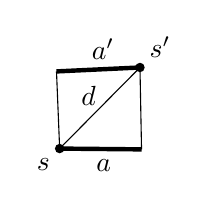
\begin{tikzpicture}[x=1cm,y=1cm]
\draw (0,.05)--(-.04,1.03) (1.04,.04)--(1.02,1.08);
\draw[line width=1.6pt](-.04,1.03)--(1.02,1.08) (0,.05)--(1.04,.04);
\draw (0,.05)--(1.02,1.08);
\fill (0,.05) circle (.06) (1.02,1.08) circle (.06);
\node[below left] at (0,.05){$s$}; \node[above right] at (1.02,1.08){$s'$};
\node[above] at (.55,1.06){$a'$}; \node[below] at (.56,.04){$a$};
\node[above left,inner sep=1pt] at (.50,.56){$d$};
\end{tikzpicture}}
tandis que $\underline\omega_Q$ s'identifie à \deleted{l'ensemble} un ensemble de deux parties de $\mathcal{R}$ (``$\mathcal{R}^+$'' et ``$\mathcal{R}^-$'') complémentaires l'une de l'autre, et stables chacune par l'antipodisme $\underline a$ (qui conserve l'orientation), ce qui fait que le choix d'un élément de $\mathcal{R}/\underline a$ définit canoniquement une orientation de $Q$, \deleted{\unsure{i.e.}} i.e. un des deux \deleted{\unsure{sous-ens.}} ens. de repères $\mathcal{R}',\mathcal{R}''$. Pour vérifier \deleted{que} si cette description d'une isom. $C\wedge D\simeq\underline\omega_Q$ i.e. d'une relation $\underline\omega_Q\wedge C\wedge D\simeq1$ correspond à $(*)$ \deleted{\unsure{$\varpi$}$\wedge c\wedge d=\unsure{0|1}$}, \inserted{$\varpi c d=1$}, il faut expliciter d'abord la convention qui nous \deleted{\unsure{fait|font}} conduit aux plongements
\[
\begin{aligned}
C&\hookrightarrow V_S\setminus\{1,\underline a\}\subset\unsure{\mathfrak{D}|\mathscr{D}},\quad D\hookrightarrow V_A\setminus\{1,\underline a\}\subset\mathfrak{D},\\
&\underline\omega_Q\subset\mathfrak{D}^+\subset\mathfrak{D}.
\end{aligned}
\]
Si $c$ est une \inserted{codiagonale i.e.} paire de côtés opposés du carré, je vais lui associer l'autom \unsure{$j_c$|$J_c$|$\gamma_c$} du carré qui fixe ces deux côtés et qui échange les deux autres i.e. la symétrie p.r. à l'axe transverse. \unsure{Dualement|Idemt|Autrement|De même}, pour une diagonale, je lui associe la symétrie par rapport à cette diagonale. Pour une orientation définie par un repère \deleted{\unsure{ce}}
\figure{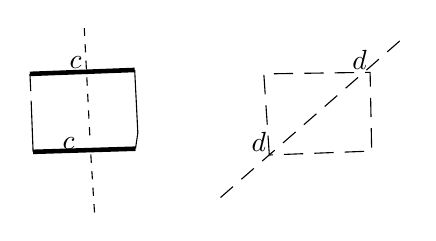
\begin{tikzpicture}[x=1cm,y=1cm]
\draw (0,.06)--(-.025,.71) (-.03,.83)--(-.04,1.05) (1.3,.1)--(1.33,.3)--(1.29,1.1);
\draw[line width=1.65pt](-.04,1.05)--(1.29,1.1) (0,.06)--(1.3,.1);
\draw[dashed](.78,-.71)--(.73,.07) (.72,.27)--(.65,1.63);
\node[above left,inner sep=.5pt] at (.64,1.09){$c$}; \node[above,inner sep=.5pt] at (.45,.07){$c$};
\begin{scope}[xshift=3cm]
\draw[dash pattern=on 7pt off 4pt](0,.02)--(-.07,1.05)--(1.28,1.07)--(1.30,.07)--(0,.02);
\draw[dash pattern=on 6pt off 4pt](-.62,-.52)--(1.75,1.55);
\node[above left,inner sep=1pt] at (0,.02){$d$}; \node[above left,inner sep=1pt] at (1.28,1.07){$d$};
\end{scope}
\end{tikzpicture}}
% archive sheet number: 12
\scanpage{14}
\figure{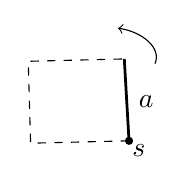
\begin{tikzpicture}[x=1cm,y=1cm]
\draw[dashed](1.25,.03)--(0,0)--(-.03,1.04)--(1.19,1.07);
\draw[line width=1pt](1.19,1.07)--(1.25,.03);
\fill(1.25,.03) circle (.052);
\node[right] at (1.25,.53){$a$}; \node[below right,inner sep=1pt] at (1.25,.03){$s$};
\draw[->](1.58,1.01)..controls (1.67,1.22) and (1.40,1.42)..(1.11,1.46);
\end{tikzpicture}}
je lui associe la rotation du carré qui transforme $s$ en le deuxième sommet de $a$. On vérifie que avec ces conventions, la formule $\varpi c d=1$ est bien la formule qui exprime que $\mathcal{R}_{\varpi}\subset \mathcal{R}$ contient l'image inverse par $\mathcal{R}\unsure{\longrightarrow|\text{---}}\mathcal{R}/\underline a$ de l'élément $(c,d)$ de $\mathcal{R}/\underline a$. Le fait que si on exprime la $=$ relation pour le carré dual, on semble obtenir le résultat opposé, provient du fait que si on identifie le $=$ ensemble $\mathcal{R}$ à l'ens. des repères de $Q$ \uline{et} de $Q^{\unsure{o|0|\circ}}$, \deleted{les} \deleted{deux} \inserted{et} le $=$ groupe $\unsure{\mathfrak{D}|\mathscr{D}}$ à $\mathrm{Aut}\,Q$ \uline{et} à $\mathrm{Aut}(Q^o)$ (ce qui n'est possible canoniquement que d'une seule façon \inserted{\unsure{raisonnable|vraisemblable}}, i.e. ce n'est pas une question de choix de conventions \ldots) alors une $=$ \deleted{partie} \inserted{classe} $\mathcal{R}'$ dans $\mathcal{R}$ \deleted{\unsure{comme|commune}} (pour la relation d'équivalence \unsure{de|del} l'orientation), considérée comme définissant une orientation de $Q$ \uline{et} une orientation de $Q^o$, définit deux orientations \uline{opposées}, en ce sens que les autom. de rotations qu'il définit via un repère $(s,a)$, suivant qu'il est regardé comme rep. de $Q$ ou rep. de $Q^o$, \unsure{sont|soit} \uline{opposés} l'un de l'autre : transformer $s$ en $s'$ ou $a$ en $a'$ se fait par deux rotations \uline{opposées}.
\figure{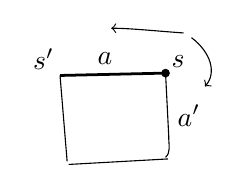
\begin{tikzpicture}[x=1cm,y=1cm]
\draw(0,.08)--(-.09,1.17) (1.25,1.20)--(1.29,.41)..controls (1.29,.27) and (1.32,.20)..(1.25,.13) (1.28,.11)--(.02,.04);
\draw[line width=1.0pt](-.09,1.17)--(1.25,1.20);
\fill(1.25,1.20) circle (.055);
\node[above left,inner sep=2pt] at (-.09,1.17){$s'$}; \node[above right,inner sep=2pt] at (1.25,1.20){$s$};
\node[above] at (.48,1.19){$a$}; \node[right] at (1.28,.66){$a'$};
\draw[->](1.48,1.71)..controls (1.18,1.73) and (.80,1.77)..(.56,1.77);
\draw[->](1.58,1.65)..controls (1.83,1.46) and (1.90,1.20)..(1.75,1.03);
\end{tikzpicture}}
% archive sheet number: 13
